%%==================================================================%%
%% Author : Abascal Fern�ndez, Patricia                             %%
%% Author : S�nchez Barreiro, Pablo                                 %%
%% Version: 1.1, 21/04/2013                                         %%
%%                                                                  %%
%% Memoria del Proyecto Fin de Carrera                              %%
%% Cap�tulo Domain Engineering, Archivo ra�z                        %%
%%==================================================================%%

\chapterheader{Ingenier�a del Dominio}{Ingenier�a del Dominio}
\label{chap:domain}

Este cap�tulo describe el proceso de desarrollo de los generadores de c�digo para la fase de \emph{Ingenier�a del Dominio} dentro de la metodolog�a Te.Net. Para ello primero describiremos las reglas que especifican c�mo se transforman los elementos del modelo a c�digo C\#. A continuaci�n,  profundizaremos en el desarrollo e implementaci�n de los generadores de c�digo. Para ilustrar c�mo funcionan los generadores de c�digo, proporcionaremos un ejemplo sencillo. Concluiremos detallando c�mo se han realizado las pruebas de los generadores de c�digo creados.

\chaptertoc

\section{Introducci�n}
\label{domain:sec:intro}

%%==================================================================%%
%% Author : Abascal Fern�ndez, Patricia                             %%
%%          S�nchez Barreiro, Pablo                                 %%
%% Version: 1.0, 14/02/2013                                         %%                                                                                    %%                                                                  %%
%% Memoria del Proyecto Fin de Carrera                              %%
%% Archivo ra�z                                                     %%
%%==================================================================%%

\chapterheader{Introducci�n}{Introducci�n}
\label{chap:introduction}

Este cap�tulo sirve de introducci�n a la presente Memoria de Proyecto Fin de Carrera. En �l se describen los objetivos generales del proyecto, as� como el contexto donde se enmarca.  Por �ltimo, se describe como se estructura el presente documento.

\chaptertoc

\section{Introducci�n}
\label{sec:intr:introduction}

%%==================================================================%%
%% Author : Sa�udo Olmedo, Ignacio                                  %%
%%          S�nchez Barreiro, Pablo                                 %%
%% Version: 2.2, 18/06/2014                                         %%                                                                                    %%                                                                  %%
%% Memoria del Proyecto Fin de Carrera                              %%
%% Introducci�n                                                     %%
%%==================================================================%%

El t�rmino conocido como modelado ha sido asociado a las bases de datos y a la gesti�n de datos durante d�cadas.
[1] El modelo entidad-relaci�n (ER) y el conjunto de reglas para la transformaci�n de un modelo ER en un esquema relacional es un ejemplo conocido y utilizado.
Recientemente  las nuevas tecnolog�as de gesti�n de datos, tambi�n conocidas como tecnolog�as NoSQL, han surgido como respuesta a los nuevos retos y demandas de las aplicaciones de Internet modernas.
Estas tecnolog�as se han centrado en el nivel de aplicaci�n, al carecer de un soporte de modelado adecuado.
Las aplicaciones de Internet emergentes, como las redes sociales (por ejemplo, Twitter) o tiendas online conocidas (por ejemplo, Amazon), est�n generando nuevos desaf�os en materia de almacenamiento y gesti�n de datos. Por ejemplo, la disponibilidad se est� convirtiendo en un aspecto critico ya que una ca�da del sistema puede generar grandes p�rdidas. Del mismo modo, estas aplicaciones tienen que soportar picos de carga altos de los usuarios, en los que estos usuarios ejecutan operaciones muy similares (por ejemplo, publicar un mensaje corto en una red social despu�s de un evento popular, como la final de la Super Bowl o unas elecciones presidenciales).

En este contexto las bases de datos relacionales tradicionales han resultado ser insuficientes para satisfacer estas nuevas exigencias. Las tecnolog�as NoSQL (Not Only SQL) [2] tienen como objetivo hacer frente a estas nuevas exigencias. NoSQL sacrifica algunas de las ventajas bien conocidas de los sistemas de gesti�n de bases de datos relacionales, como la integridad o la manipulaci�n de transacciones, con el fin de proporcionar una mejor escalabilidad y un mayor rendimiento. Siguiendo esta idea, varios sistemas NoSQL, como Cassandra [3], HBase [4] o MongoDB [5], han aparecido en los �ltimos a�os.

Sin embargo, las tecnolog�as NoSQL no est�n a�n integradas en los procesos de desarrollo de software que ayudan a los ingenieros de software en la construcci�n de repositorios NoSQL desde las primeras etapas del ciclo de vida del software hasta el lanzamiento del producto. Este trabajo tiene como objetivo contribuir con una herramienta para superar esta barrera, proporcionando una herramienta que genera bases de datos NoSQL.

Por lo tanto, este trabajo se centrar� en la creaci�n de un generador de c�digo que transforma un modelo de datos conceptual UML en c�digo para la creaci�n de un repositorio de datos NoSQL. Para este trabajo, nos centraremos en los sistemas orientados a columnas. Las razones son las siguientes: (1) sistemas orientados a columnas son de uso general, mientras que otros sistemas NoSQL, tales como, los de gesti�n de documentos, son m�s espec�ficos a ese dominio; y, (2) que ten�a experiencia previa en el manejo de estos sistemas. M�s concretamente, hemos decidido utilizar Cassandra [3] como sistema NoSQL orientado a columnas debido a su creciente popularidad.

El modelado de datos de un sistema como Cassandra dista del modelado tradicional de las bases de datos relacionales. Cassandra por ejemplo utiliza como unidad b�sica las Columns cuyo equivalente seria el Campo en el modelo relacional o como unidad de almacenamiento de las Columns utiliza las ColumnFamily como tablas etc..

Para realizar este generador de c�digo se utilizan una serie de t�cnicas de transformaci�n entre modelos conocidas como "Desarrollo Dirigido por Modelos" (MDD). MDD se puede definir como  un enfoque de la Ingenier�a del software y de la Ingenier�a dirigida por modelos (MDE) que utiliza el modelo para crear un producto. �Y que es un modelo?. Un modelo se puede entender como la descripci�n o representaci�n de un sistema en un lenguaje bien definido.
Para entender lo que representa un modelo dentro de MDE hay que saber previamente lo que es un meta-modelo. Un meta-modelo es un modelo usado para especificar un lenguaje, b�sicamente describe las caracter�sticas del lenguaje. Por lo tanto un modelo se puede entender como la instancia de un meta-modelo. Estos conceptos son ampliados en siguientes secciones.

El resultado de la utilizaci�n de MDD es traducido en reducci�n de costes debido a que el recurso humano requerido es menor, un aumento de la productividad y reutilizaci�n de componentes adem�s se puede aumentar el nivel de abstracci�n a la hora de realizar el dise�o de un software.

En resumen la utilizaci�n de modelos UML respecto a modelos escritos en Cassandra a la hora de especificar una base de datos no relacional proporciona una abstracci�n para aquellos usuarios que no est�n muy familiarizados con el modelado de bases de datos no relacionales. La utilizaci�n de modelos dise�ados en UML proporciona ventajas ya que UML es un lenguaje de modelado bien conocido por toda la comunidad. Adem�s la automatizaci�n de estos procesos nos permite crear software m�s r�pido, m�s fiable y de mayor calidad lo que nos lleva a mantener buenas pr�cticas. Este trabajo pretende contribuir a satisfacer las carencias y virtudes citadas, proporcionando una herramienta que bajo las bases de un proceso de transformaci�n dirigido por modelos transforma y genera keyspaces para sistemas NoSQL orientado a columnas. Esperamos que esto permita a los equipos de desarrollo ahorrar esfuerzos y, por lo tanto, reducir costes.

En las siguientes secciones se desarrollan los siguientes aspectos: El apartado 1.2 expande informaci�n sobre la Ingenier�a dirigida por modelos y el Desarrollo Dirigido por Modelos, este apartado es vital para entender todo lo relacionado con la memoria presente. El apartado 1.3 presenta la motivaci�n y objetivos del proyecto. Finalmente el apartado 1.4 describe la estructura que tendr� el documento presente.











\section{Planificaci�n del proyecto}
\label{sec:intr:planning}

% %%==================================================================%%
%% Author : Tejedo Gonz�lez, Daniel                                 %%
%%          S�nchez Barreiro, Pablo                                 %%
%% Version: 1.0, 22/11/2012                                         %%
%% Version: 2.0, 31/01/2013                                         %%
%%                                                                  %%
%% Memoria del Proyecto Fin de Carrera                              %%
%% Planificacion, planificacion                                     %%
%%==================================================================%%

Como se ha comentado con anterioridad, el objetivo de este Proyecto Fin de Carrera es el desarrollo de un editor para un novedoso lenguaje de especificaci�n y validaci�n de restricciones para �rboles de caracter�sticas donde dichas restricciones puedan incluir caracter�sticas clonables. Dicho editor se desarrollar� utilizando un moderno enfoque de \emph{Ingenier�a de Lenguajes Dirigido por Modelos}. Por tanto, el proceso de desarrollo del presente proyecto queda pr�cticamente determinado por dicho enfoque, el cual posee un proceso de desarrollo bien definido, el cual se describi� en la secci�n anterior. La Figura~\ref{fig:planning} muestra como dicho proceso de desarrollo se ha instanciado para nuestro caso particular.

%%==================================================================%%
%% NOTA(Pablo): En esta imagen hay que hacer cambios                %%
%%              Te los indico de foma verbal cuando pases por el    %%
%%              despacho, pero hay que mejorar su consistencia      %%
%%==================================================================%%

\begin{figure}[!tb]
    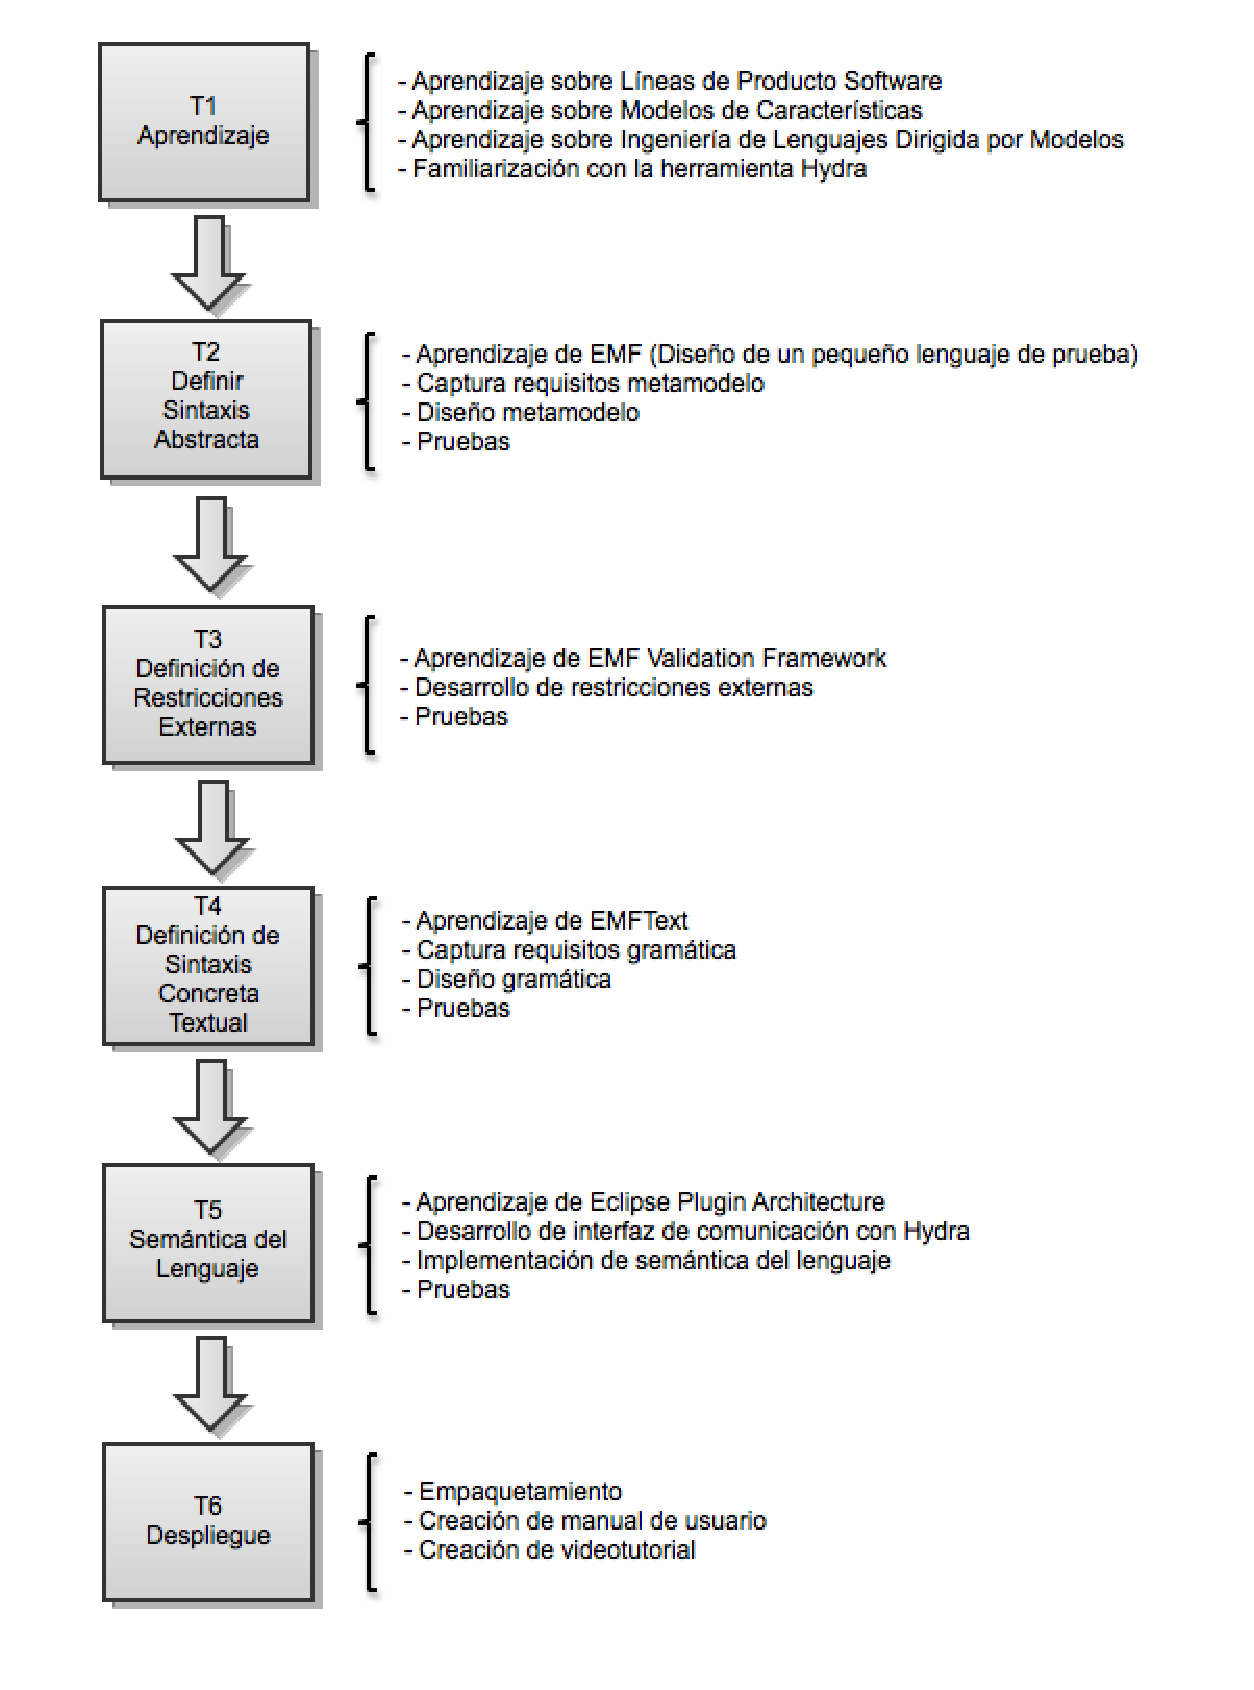
\includegraphics[scale=0.74]{planificacion/planning.eps}
    \caption{Proceso de desarrollo del Proyecto Fin de Carrera}
    \label{fig:planning}
\end{figure}

Obviamente, la primera tarea (Figura~\ref{fig:planning}-\emph{T1}) en este proceso de desarrollo fue la de adquirir los conocimientos necesarios para la realizaci�n de todas las tareas posteriores. Ello implicaba adquirir los conocimientos relacionados con las \emph{L�neas de Producto Software}~\cite{} en general y con los �rboles de caracter�sticas~\cite{} en particular, m�s concretamente, con la vesi�n de los �rboles de caracter�sticas que soportan la definici�n de caracter�sticas clonables~\cite{}. Dado que el proyecto se deb�a integrar con una herramienta para la especificaci�n y configuraci�n de �rboles de caracter�sticas concreta, denominada \emph{Hydra}~\cite{}, el siguiente paso fue el de familiarizarse con dicha herramienta y adquirir ciertos conocimientos sobre su arquitectura interna.

A continuaci�n, se tuvo que adquirir los conceptos necesarios para entender el funcionamiento de de la \emph{Ingenier�a de Lenguajes Dirigida por Modelos}~\cite{}. La familiarizaci�n con las tecnolog�as concretas relacionadas con la \emph{Ingenier�a de Lenguajes Dirigida por Modelos}, como la utilizaci�n de EMF (\emph{Eclipse Modelling Framework})~\cite{} para la definici�n de metamodelos, se realiz� dentro de cada fase concreto del proyecto, a medida que se iba necesitando aprender a utilizar dichas tecnolog�as.

%%========================================================================================%%
%% NOTA(Pablo): No pongas los tiempos que te ha costado cada tarea. Normalmente, no
%%              interesa y da mala imagen
%%========================================================================================%%

Tras esta tarea inicial de adquisici�n de conocimientos previos, el resto del proyecto se estructura como un proyecto de desarrollo de un lenguaje software siguiendo un enfoque dirigido por modelos. Consecuentemente, la primera tarea tras la fase inicial de documentaci�n (Figura~\ref{fig:planning}-\emph{T2}) fue la definici�n de la sintaxis abstracta, por medio de un metamodelo m�s un conjunto de restricciones externas, para el lenguaje que deb�a soportar nuestro editor. Para ello tuvimos que capturar los requisitos que deb�a satisfacer dicho lenguaje. Tras recoger dichos requisitos, se procedi� al dise�o del metamodelo y a la relizaci�n de las pruebas pertinentes con vistas a comprobar su correcto funcionamiento. Para crear dicho metamodelo se utiliz� el lenguaje de metamodelado Ecore, integrado dentro de la herramienta EMF (Eclipse Modelling Framework)~\cite{}.

A continuaci�n, de acuerdo con los expuesto en la secci�n anterior, procedimos a definir la las restricciones externas que no pod�an ser definidas en Ecore (Figura~\ref{fig:planning}-\emph{T3}). Dichas restricciones se implementaron utilizando la facilidad de EMF denominada EMF Validation Framework~\cite{}.

A continuaci�n, procedimos a definir la sintaxis concreta, en nuestro caso textual, para nuestro lenguaje de modelado. Optamos por una sintaxis textual ya que las restricciones a especificar son una especie de f�rmulas l�gicas, las cuales resultan m�s c�modas de especificar mediante notaciones textuales que mediante notaciones gr�ficas (Figura~\ref{fig:planning}-\emph{T4}). Para el desarrollo de dicha sintaxis textual hubo que hacer un nuevo an�lisis de los requisitos que dicha notaci�n textual deb�a satisfacer. A continuaci�n se especific� la gram�tica de nuestra sintaxis textual, ligando sus elementos con los del metamodelo producido en la fase anterior y se ejecutaron los casos de prueba necesarios para comprobar su correcto funcionamiento. Para crear dicha sintaxis textual se utiliz� la herramienta EMFText~\cite{}.

Las etapas anteriores permit�an disponer de un editor que soportaba la especificaci�n de restricciones de acuerdo al lenguaje HCL. Por tanto, s�lo restaba poder comprobar, para una configuraci�n dada de un �rbol de caracter�sticas, que dichas restricciones se satisfac�an. Ello implicaba dotar de sem�ntica al lenguaje y, a partir de dicha sem�ntica, implementar los mecanismos necesarios para la comprobaci�n de la validez de dichas restricciones. La sem�ntica del lenguaje ya estaba definida por el profesor Pablo S�nchez, por lo que s�lo hubo que implementar el c�digo necesario para procesar un modelo de restricciones y comprobar que dichas restricciones se satisfac�an. Dicho c�digo se implement� en Java, utilizando las facilidades que el entorno EMF proporciona para la manipulaci�n del modelo  (Figura~\ref{fig:planning}-\emph{T5}). Para poder implementar la sem�ntica, fue necesario crear una interfaz de comunicaci�n con la herramienta \emph{Hydra} que permitiese conocer el estado en el cual se hallaba cada caracter�stica. Tras la implementaci�n, se ejecut� un exhaustivo conjunto de pruebas para comprobar el correcto funcionamiento del c�digo creado.

En este punto del proceso de desarrollo ten�amos implementado el editor requerido, por lo que s�lo restaba proceder a su despliegue (Figura~\ref{fig:planning}-\emph{T6}). Este despliegue implicaba su integraci�n dentro de la arquitectura de plugins de Eclipse y, m�s concretamente, de la herramienta \emph{Hydra}. Tras dicha integraci�n, se procedi� a realizar una serie de pruebas de aceptaci�n, destinadas a comprobar que el trabajo realizado satisfac�a las necesidades de los usuarios finales que iban a utilizar el editor creado.



\section{Estructura del Documento}
\label{sec:intr:estructura}

% %%==================================================================%%
%% Author : Tejedo Gonz�lez, Daniel                                 %%
%%          S�nchez Barreiro, Pablo                                 %%
%% Version: 1.0, 22/11/2012                                         %%
%% Version: 2.0, 31/01/2013                                         %%
%%                                                                  %%
%% Memoria del Proyecto Fin de Carrera                              %%
%% Planificacion, planificacion                                     %%
%%==================================================================%%

Como se ha comentado con anterioridad, el objetivo de este Proyecto Fin de Carrera es el desarrollo de un editor para un novedoso lenguaje de especificaci�n y validaci�n de restricciones para �rboles de caracter�sticas donde dichas restricciones puedan incluir caracter�sticas clonables. Dicho editor se desarrollar� utilizando un moderno enfoque de \emph{Ingenier�a de Lenguajes Dirigido por Modelos}. Por tanto, el proceso de desarrollo del presente proyecto queda pr�cticamente determinado por dicho enfoque, el cual posee un proceso de desarrollo bien definido, el cual se describi� en la secci�n anterior. La Figura~\ref{fig:planning} muestra como dicho proceso de desarrollo se ha instanciado para nuestro caso particular.

%%==================================================================%%
%% NOTA(Pablo): En esta imagen hay que hacer cambios                %%
%%              Te los indico de foma verbal cuando pases por el    %%
%%              despacho, pero hay que mejorar su consistencia      %%
%%==================================================================%%

\begin{figure}[!tb]
    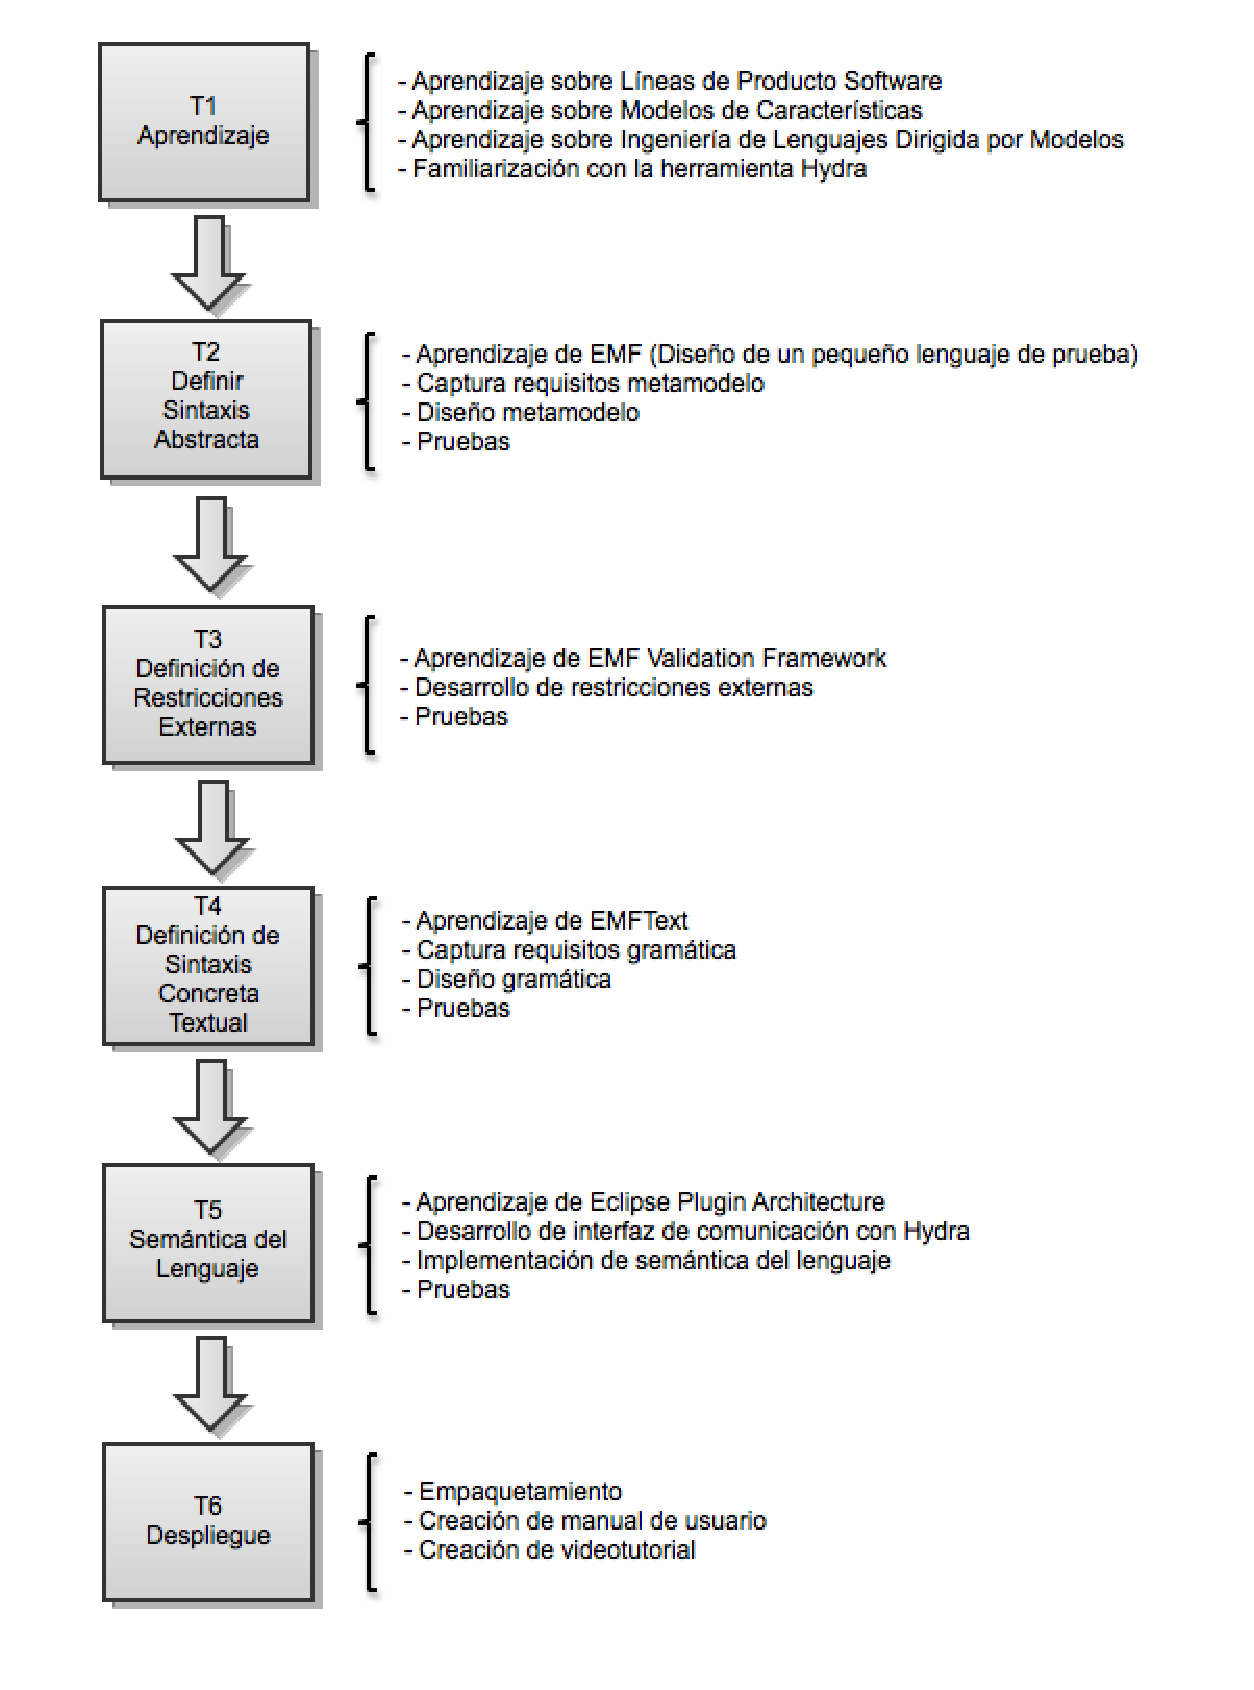
\includegraphics[scale=0.74]{planificacion/planning.eps}
    \caption{Proceso de desarrollo del Proyecto Fin de Carrera}
    \label{fig:planning}
\end{figure}

Obviamente, la primera tarea (Figura~\ref{fig:planning}-\emph{T1}) en este proceso de desarrollo fue la de adquirir los conocimientos necesarios para la realizaci�n de todas las tareas posteriores. Ello implicaba adquirir los conocimientos relacionados con las \emph{L�neas de Producto Software}~\cite{} en general y con los �rboles de caracter�sticas~\cite{} en particular, m�s concretamente, con la vesi�n de los �rboles de caracter�sticas que soportan la definici�n de caracter�sticas clonables~\cite{}. Dado que el proyecto se deb�a integrar con una herramienta para la especificaci�n y configuraci�n de �rboles de caracter�sticas concreta, denominada \emph{Hydra}~\cite{}, el siguiente paso fue el de familiarizarse con dicha herramienta y adquirir ciertos conocimientos sobre su arquitectura interna.

A continuaci�n, se tuvo que adquirir los conceptos necesarios para entender el funcionamiento de de la \emph{Ingenier�a de Lenguajes Dirigida por Modelos}~\cite{}. La familiarizaci�n con las tecnolog�as concretas relacionadas con la \emph{Ingenier�a de Lenguajes Dirigida por Modelos}, como la utilizaci�n de EMF (\emph{Eclipse Modelling Framework})~\cite{} para la definici�n de metamodelos, se realiz� dentro de cada fase concreto del proyecto, a medida que se iba necesitando aprender a utilizar dichas tecnolog�as.

%%========================================================================================%%
%% NOTA(Pablo): No pongas los tiempos que te ha costado cada tarea. Normalmente, no
%%              interesa y da mala imagen
%%========================================================================================%%

Tras esta tarea inicial de adquisici�n de conocimientos previos, el resto del proyecto se estructura como un proyecto de desarrollo de un lenguaje software siguiendo un enfoque dirigido por modelos. Consecuentemente, la primera tarea tras la fase inicial de documentaci�n (Figura~\ref{fig:planning}-\emph{T2}) fue la definici�n de la sintaxis abstracta, por medio de un metamodelo m�s un conjunto de restricciones externas, para el lenguaje que deb�a soportar nuestro editor. Para ello tuvimos que capturar los requisitos que deb�a satisfacer dicho lenguaje. Tras recoger dichos requisitos, se procedi� al dise�o del metamodelo y a la relizaci�n de las pruebas pertinentes con vistas a comprobar su correcto funcionamiento. Para crear dicho metamodelo se utiliz� el lenguaje de metamodelado Ecore, integrado dentro de la herramienta EMF (Eclipse Modelling Framework)~\cite{}.

A continuaci�n, de acuerdo con los expuesto en la secci�n anterior, procedimos a definir la las restricciones externas que no pod�an ser definidas en Ecore (Figura~\ref{fig:planning}-\emph{T3}). Dichas restricciones se implementaron utilizando la facilidad de EMF denominada EMF Validation Framework~\cite{}.

A continuaci�n, procedimos a definir la sintaxis concreta, en nuestro caso textual, para nuestro lenguaje de modelado. Optamos por una sintaxis textual ya que las restricciones a especificar son una especie de f�rmulas l�gicas, las cuales resultan m�s c�modas de especificar mediante notaciones textuales que mediante notaciones gr�ficas (Figura~\ref{fig:planning}-\emph{T4}). Para el desarrollo de dicha sintaxis textual hubo que hacer un nuevo an�lisis de los requisitos que dicha notaci�n textual deb�a satisfacer. A continuaci�n se especific� la gram�tica de nuestra sintaxis textual, ligando sus elementos con los del metamodelo producido en la fase anterior y se ejecutaron los casos de prueba necesarios para comprobar su correcto funcionamiento. Para crear dicha sintaxis textual se utiliz� la herramienta EMFText~\cite{}.

Las etapas anteriores permit�an disponer de un editor que soportaba la especificaci�n de restricciones de acuerdo al lenguaje HCL. Por tanto, s�lo restaba poder comprobar, para una configuraci�n dada de un �rbol de caracter�sticas, que dichas restricciones se satisfac�an. Ello implicaba dotar de sem�ntica al lenguaje y, a partir de dicha sem�ntica, implementar los mecanismos necesarios para la comprobaci�n de la validez de dichas restricciones. La sem�ntica del lenguaje ya estaba definida por el profesor Pablo S�nchez, por lo que s�lo hubo que implementar el c�digo necesario para procesar un modelo de restricciones y comprobar que dichas restricciones se satisfac�an. Dicho c�digo se implement� en Java, utilizando las facilidades que el entorno EMF proporciona para la manipulaci�n del modelo  (Figura~\ref{fig:planning}-\emph{T5}). Para poder implementar la sem�ntica, fue necesario crear una interfaz de comunicaci�n con la herramienta \emph{Hydra} que permitiese conocer el estado en el cual se hallaba cada caracter�stica. Tras la implementaci�n, se ejecut� un exhaustivo conjunto de pruebas para comprobar el correcto funcionamiento del c�digo creado.

En este punto del proceso de desarrollo ten�amos implementado el editor requerido, por lo que s�lo restaba proceder a su despliegue (Figura~\ref{fig:planning}-\emph{T6}). Este despliegue implicaba su integraci�n dentro de la arquitectura de plugins de Eclipse y, m�s concretamente, de la herramienta \emph{Hydra}. Tras dicha integraci�n, se procedi� a realizar una serie de pruebas de aceptaci�n, destinadas a comprobar que el trabajo realizado satisfac�a las necesidades de los usuarios finales que iban a utilizar el editor creado.






\section{Transformaciones de Modelo UML a C\#}
\label{domain:sec:transf}

%%==================================================================%%
%% Author : Abascal Fern�ndez, Patricia                             %%
%% Author : S�nchez Barreiro, Pablo                                 %%
%% Version: 1.4, 29/04/2013                                         %%
%%                                                                  %%
%% Memoria del Proyecto Fin de Carrera                              %%
%% Domain Engineering/Transformaci�n UML a C#                       %%
%%==================================================================%%

Como hemos comentado, el primer paso para desarrollar una transformaci�n de modelo a c�digo es: (1) identificar los distintos casos o tipos de entrada con los que nos podemos encontrar; y (2) hallar un equivalente en el lenguaje destino (C\# en nuestro caso). A continuaci�n, mostramos los casos identificados (c�mo t�tulo de cada subsecci�n), y por cada caso, comentamos las equivalencias propuestas. Ciertas de estas reglas son espec�ficas para l�neas de productos software, mientras que otras, como la transformaci�n de las asociaciones, son aplicables a cualquier transformaci�n de UML 2.0 a C\#.
Cada regla de transformaci�n la ilustramos utilizando el ejemplo de la Figura~\ref{back:fig:smartHome}.

\subsection{Modelo}

Un modelo UML, es decir, el elemento ra�z que contiene al resto de los elementos de un modelo UML, se transforma en el \emph{namespace} para el proyecto C\#. Los \emph{namespaces} permiten agrupar entidades tales como paquetes, clases, objetos y funciones bajo el mismo nombre. De esta forma, se pueden tener varios \emph{namespaces} en el mismo proyecto que son independientes entre s�.

Recordar que para que varias clases parciales puedan ser combinadas, �stas deben pertenecer a un mismo \emph{namespace}. Por tanto, se utiliza como nombre de dicho \emph{namespace}, el nombre del modelo UML 2.0 que sirve de entrada a los generadores de c�digo.

Adem�s, al transformar el modelo UML 2.0, se crea un proyecto Visual Studio 2010, inicialmente vac�o, con el mismo nombre que el modelo UML 2.0.

Para el caso de la Figura~\ref{back:fig:smartHome}, el nombre del modelo, el cual no aparece en el diagrama, es \emph{SmartHome}. Por tanto, se crear�a un proyecto Visual Studio 2010, con \emph{SmartHome} como nombre. Dentro de dicho proyecto, se crear�a un \emph{namespace} denominado \emph{SmartHome}.

\subsection{Paquete}

Cada paquete UML 2.0 representa en nuestro caso una familia de clases, la cual encapsula una caracter�stica. Por tanto, por cada paquete UML 2.0, se crea una nueva carpeta o directorio, con el mismo nombre que el paquete, en el proyecto Visual Studio 2010 creado al transformar el modelo que contiene dicho paquete. En dicho directorio se colocar�n todos los ficheros resultantes de transformar el contenido de dicho paquete.

Por ejemplo, para el caso de la Figura~\ref{back:fig:smartHome}, durante la transformaci�n del paquete \imp{WindowMng}, se crear�a una nueva carpeta dentro del proyecto Visual Studio 2010 generado, denominada \imp{WindowMng}. Lo mismo se aplicar�a al resto de los paquetes.

\subsection{Tipos primitivos}
\label{subsec:domain:primitiveType}

Por cada tipo primitivo de UML 2.0, se establece una correspondencia con los tipos primitivos de C\#. Por ejemplo, un \emph{String} de UML 2.0 se transforma en \emph{String} de C\#. Un \emph{boolean} de UML 2.0 se transforma en un \emph{bool} de C\#. Esta correspondencia es bastante directa y no presenta problemas m�s de all� de tener que renombrar algunos tipos.

\subsection{Clases Enumeradas}

Cada clase enumerada UML 2.0, se transforma en un enumerado de C\#, con el mismo nombre que el enumerado UML 2.0. A continuaci�n, se procesan los literales de la clase enumerado UML 2.0, a�adiendo un literal con el mismo nombre al enumerado creado en C\#.

Por ejemplo, la clase enumerada \imp{TempUnits} de la caracter�stica \imp{HeaterMng} se transformar�a en un enumerado de C\#, con nombre \imp{TempUnits}, perteneciente al \emph{namespace} \imp{HeaterMng}, y con \imp{CELSIUS} y \imp{FARENHEIT} como literales. El Listado~\ref{dom:code:enum} muestra el c�digo resultante de esta transformaci�n.

\begin{lstlisting} [basicstyle=\ttfamily\scriptsize,language=CSharp, captionpos=b,
                    caption=C�digo generado para la clase enumerada \imp{TempUnits},
                    label=dom:code:enum]
01 namespace SmartHome{
02    enum TempUnits {
03        CELSIUS,
04        FARENHEIT
05    };
06 }
\end{lstlisting}

\subsection{Clase}
\label{subsec:domain:class}

Por cada clase UML 2.0 encontrada dentro de un paquete, se genera una clase parcial sita en el directorio correspondiente al paquete al cual pertenece. El nombre de la clase parcial es el mismo que el de la clase UML 2.0.

Por ejemplo, para la clase \emph{WindowCtrl}, del paquete \emph{WindowMng}, se crear�a una clase parcial p�blica, denominada \emph{WindowCtrl}, y sita en la carpeta del proyecto \emph{WindowMng}.

A continuaci�n, se procesan los contenidos de dicha clase, tal como se describe a continuaci�n.

\subsection{Atributo}
\label{subsec:domain:atrib}

Cada atributo de una clase en UML 2.0 se transforma en una propiedad de C\#, perteneciente a clase parcial correspondiente a la clase que posee el atributo en el modelo UML 2.0. Dicha propiedad tendr� siempre visibilidad \emph{protegida} (\emph{protected}), salvo que estuviese declarada como \emph{privada} (\emph{private}) en el modelo UML 2.0, en cuyo caso se mantendr� la visibilidad privada.

Si el atributo era p�blico en el modelo UML, se le generar�n m�todos de acceso (\emph{getter} y \emph{setter}) a dicha propiedad. Si el atributo fuese de solo lectura o derivado, no se le generar�a m�todo de escritura (\emph{setter}).

Si el atributo fuese est�tico (\emph{static}), se generar� como est�tico en el c�digo C\#, y no se le generar�n m�todos de acceso.

Si el tipo del atributo es un tipo primitivo y el atributo no es multivaluado, es decir, la cota superior de su multiplicidad es igual a 1, se utiliza como tipo su correspondiente en C\#, de acuerdo las correspondencias comentadas en la Secci�n~\ref{subsec:domain:primitiveType}. Si el tipo fuese una clase u otro tipo no primitivo, el tipo ser� el nombre resultante de transformar dicho elemento no primitivo.

Por ejemplo, el atributo \imp{id} de la clase \imp{Actuator}, dentro de la caracter�stica \imp{BaseSystem}, se transformar�a en una propiedad llamada \imp{id}, de la clase \imp{Actuator}, sita en la carpeta \imp{BaseSystem}, y perteneciente al \emph{namespace} \imp{SmartHome}. Como tipo para dicha propiedad, se utilizar�a \imp{Int}.

Para el caso del atributo \imp{units} de la clase \imp{Actuator}, dentro de la caracter�stica \imp{HeaterMng}, se utilizar�a como tipo \imp{TempUnits}, ya que ser�a �ste el nombre del enumerado resultante de transformar la clase enumerada que sirve como tipo de este atributo.

Si el atributo fuese un atributo un atributo multivaluado, es decir, la cota superior de su multiplicidad es superior a 1, el tipo de la propiedad generada ser� una colecci�n que use como tipo base el tipo del atributo. Dependiendo de ciertas propiedades del atributo \imp{isOrdered} e \imp{isUnique}, se deber� utilizar un tipo de colecci�n u otro:

\begin{itemize}
  \item Si el atributo tiene la propiedad \imp{isOrdered=false} e \imp{isUnique=false} estamos ante una colecci�n que admite elementos repetidos y donde la posici�n es irrelevante. Se trata por tanto de una bolsa, que en C\# se representan por medio de una \imp{ICollection}.
  \item Si el atributo tiene la propiedad \imp{isOrdered=false} e \imp{isUnique=true}, se trata de un conjunto, ya que no hya repetidos y la posici�n es irrelevante. Escogemos por tanto el tipo de C\#, \imp{ISet}.
  \item Si el atributo tiene la propiedad \imp{isOrdered=true} e \imp{isUnique=false} se corresponde se tratar�a lista (\imp{IList}), ya que son elementos en los que el orden es relevante y admite repeticiones.
  \item Si el atributo tiene la propiedad \imp{isOrdered=true} e \imp{isUnique=true} estamos ante un caso raro, poco utilizado dentro del mundo del desarrollo software, y para el que no se conocen equivalencias en lenguaje C\#. Se tratar�a de una lista sin repeticiones. Se utiliza por tanto como colecci�n una lista (\imp{IList}) informando al usuario final, para que tome las medidas que considere adecuadas de cara al control de los duplicados.
\end{itemize}

\subsection{Extremos de asociaci�n}

Las asociaciones en UML pueden ser de dos tipos:

\begin{figure}[!tb]
  \centering
  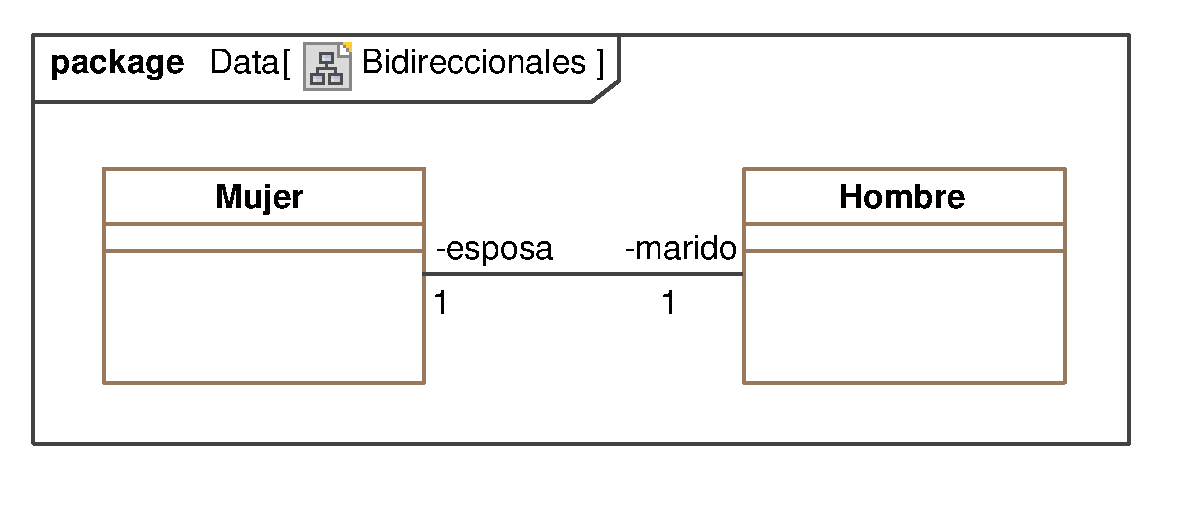
\includegraphics[width=.55\linewidth]{domainEngineering/images/transfBidirec.eps} \\
  \caption{Ejemplo de asociaci�n bidireccional}
  \label{dom:fig:transfBidirec}
\end{figure}

\begin{description}
  \item[Unidireccionales] S�lo un extremo de la asociaci�n aparece nombrado, y destacado con una flecha. Dicho extremo act�a como referencia entre clases. Por ejemplo, \imp{indoorTherm} (Figura~\ref{back:fig:smartHome}, paquete \imp{SmartEnergyMng}) representa un referencia de la clase \imp{Gateway} a la clase \imp{ThermometerCtrl}. Dichas referencias pueden referirse a un solo objeto, como el caso de \imp{indoorTherm}, o a una colecci�n de ellos, como el caso ed \imp{actuators} en la caracter�stica \imp{BaseSystem}.
  \item[Bidireccionales] Son los casos donde ambos extremos aparecen nombrados, pero no hay flechas en ninguno de los dos extremos. No se aprecian ejemplos de este tipo nuestro caso de estudio (Figura~\ref{back:fig:smartHome}), por lo que se proporciona un ejemplo adicional (ver Figura~\ref{back:fig:transfBidirec}), el cual describimos a continuaci�n. En este caso, un objeto de tipo \imp{Mujer} posee una referencia \imp{marido} a un objeto de tipo \imp{Hombre}. A su vez, un objeto de tipo \imp{Hombre} posee una referencia \imp{esposa} a un objeto de tipo \imp{Mujer}. Se espera que ambas referencias est�n relacionadas. Es decir, si un objeto \imp{m} de tipo \imp{Mujer} tiene una referencia a un objeto \imp{h} de tipo \imp{Hombre}, de acuerdo la restricci�n de integridad impuesta por las asociaciones bidireccionales, el objeto \imp{h} debe tener como valor para su referencia \imp{esposa} el objeto \imp{m} de tipo \imp{Mujer}. Dicho de forma m�s f�cil de entender, si \imp{h} est� casado con \imp{m}, \imp{m} debe de estar casado con \imp{h}.
\end{description}

En cualquier caso, los extremos de asociaci�n navegables en UML 2.0 representan referencias entre clases. Por tanto, un extremo de asociaci�n tiene el mismo tratamiento que el de un atributo, siendo su tipo es una clase. De esta forma, cada extremo navegable de una asociaci�n entre clases en UML 2.0 se transforma en una propiedad en C\#, siguiendo un tratamiento similar al de los atributos.
Al igual que en los atributos de las clases, si el extremo de asociaci�n tiene multiplicidad superior igual a 1, se utiliza la clase referenciada como tipo de la propiedad. Si la multiplicidad fuese superior a 1, se utiliza una colecci�n, siguiendo el mismo procedimiento que para los atributos, utilizando la clase referenciada como tipo base.

%%=====================================================================%%
%% NOTA(Pablo): Comenta aqu� que facilidades adicionales se generan    %%
%%              para las asociaciones bidireccionales                  %%                      %%=====================================================================%%

Adem�s, para el caso de las asociaciones bidireccionales, se genera cierta l�gica adicional, la cual est� encargada de mantener la restricci�n de integridad impuesta por la bidireccionalidad.


\section{Generadores de C�digo C\#}
\label{domain:sec:gen}

%%==================================================================%%
%% Author : Abascal Fern�ndez, Patricia                             %%
%% Author : S�nchez Barreiro, Pablo                                 %%
%% Version: 2.9, 25/04/2013                                         %%
%%                                                                  %%
%% Memoria del Proyecto Fin de Carrera                              %%
%% Domain Engineering/Generadores de C�digo C#                      %%
%%==================================================================%%

Para implementar los generadores de c�digo, se procedi� en encapsular cada una de las reglas descritas en la secci�n anterior en un \emph{template} de EGL. Adem�s, se crearon una serie de funciones auxiliares en EOL. Por ejemplo, se cre� una funci�n auxiliar para determinar el tipo de colecci�n que debe ser utilizada para transformar un atributo multivaluado, es decir, con cota superior de su multiplicidad mayor que uno.

Uno de los mayores problemas que normalmente plantean los generadores de c�digo es que la generaci�n de c�digo es secuencial, no permitiendo la vuelta a atr�s. Por ejemplo, si generamos una clase y m�s tarde descubrimos que dicha clase debe ser modificada porque act�a como clase padre en una herencia m�ltiple, ya no podremos volver a abrir dicha clase para a�adirle la relaci�n de herencia con la interfaz que ha de crearse.

Por tanto, antes de generar una clase, debemos asegurarnos de que no va a necesitar ser modificada posteriormente. Ello implica que hay que tener especial cuidado a la hora de dise�ar el orden en el cual se ejecutan las plantillas, o \emph{templates} de generaci�n de c�digo. La Figura~\ref{dom:fig:templates} muestra el orden de ejecuci�n de las plantillas creadas en nuestro caso. Explicamos parte de dicha figura, aunque no la describiremos entera, por razones de espacio.

\begin{figure}[!tb]
  \centering
  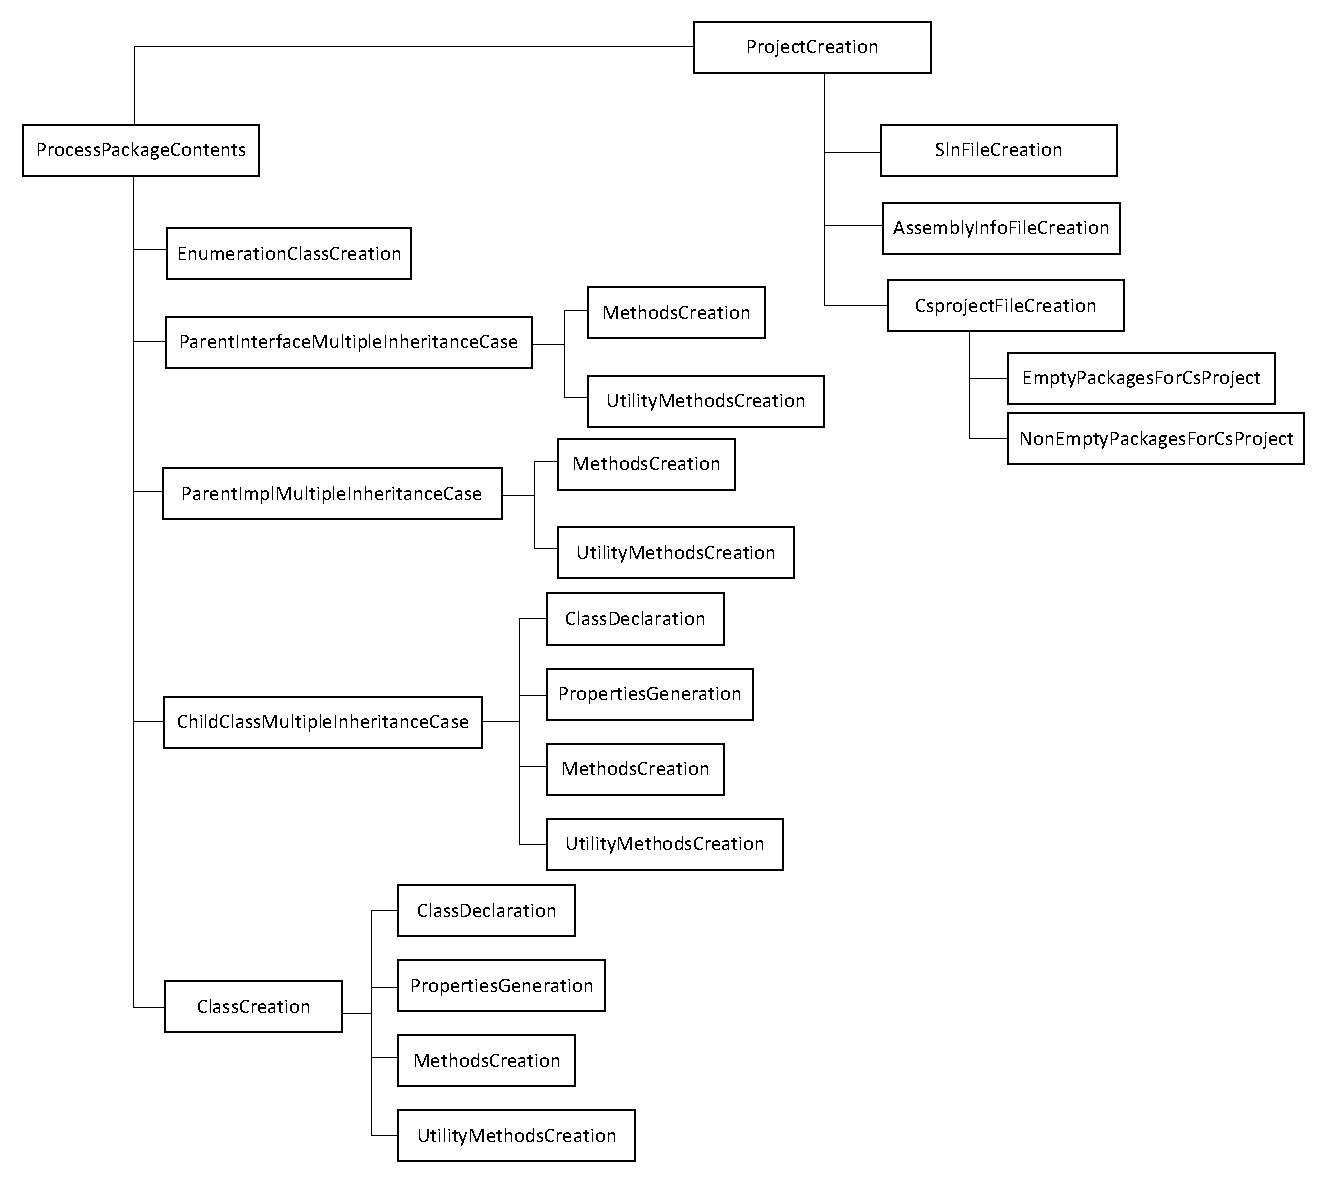
\includegraphics[width=0.9\linewidth]{domainEngineering/images/Templates.eps} \\
  \caption{Orden de ejecuci�n de las plantillas de generaci�n de c�digo}
  \label{dom:fig:templates}
\end{figure}

El punto de partida es el generador de c�digo llamado \imp{ProjectCreation}, encargado de procesar el elemento \emph{modelo}, que constituye la ra�z del proyecto, as� como los \emph{paquetes} que contiene dicho modelo, adem�s de crear el proyecto \emph{Visual Studio 2010} que constituye la salida del generador.  Dicho \emph{template} tiene , por tanto, dos tareas claramente diferenciadas: (1) por una parte, debe generar el c�digo correspondiente a la arquitectura de referencia, lo que se hace a trav�s de la plantilla \imp{ClassFilesCreation}; y (2) por otra parte, debe generar todos los ficheros auxiliares y la estructura que constituyen un proyecto \emph{Visual Studio 2010}, como el fichero de construcci�n (fichero \emph{.csproj}) que indica que clases parciales deben compilarse cuando se construye el proyecto (ver Figura~\ref{back:code:partialClasses}). Para generar estos ficheros auxiliares, se utilizan las plantillas \imp{SlnFileCreation},  \imp{CsprojectFileCreation} y \imp{AssemblyInfoFileCreation}.

La plantilla \imp{ProcessPackageContents} procesa por cada paquete, su contenido. Dependiendo del tipo de cada elemento, se realiza una acci�n diferente, tal como se describe a continuaci�n.

Si se trata de una clase enumerada, se invoca el template \imp{EnumerationClassCreation}, con dicho elemento como argumento.

Se procesan todas las clases con herencia m�ltiple, para aplicar el \emph{mixin pattern}. Para ello se ejecutan las plantillas \imp{ParentImplMultipleInheritanceCase}, que se encarga de procesar las clases padre involucradas en herencias m�ltiples; y \imp{ParentInterfaceMultipleInheritanceCase}, que se encarga de crear las interfaces para estas clases padre. Ambas plantillas hacen uso de las plantillas \imp{MethodsCreation} y \imp{UtilityMethodsCreation}, encargadas de procesar los m�todos de dichas clases e interfaces y de crear los m�todos de infraestructura que fuesen necesarios, tal como \imp{Equals} o \imp{CompareTo}.

A continuaci�n, se ejecuta la plantilla \imp{ChildClassMultipleInheritance}, encargada de procesar una clase hija involucrada en herencia m�ltiple. Para ello se procesan el esqueleto de la clase (\imp{ClassDeclaration}), sus atributos (\imp{PropertiesGeneration}), sus m�todos (\imp{MethodsCreation}) y sus m�todos de infraestructura (\imp{UtilityMethodsCreation}).

Seguidamente, se procesan las clases no afectadas, como hijas o como padres, por herencia m�ltiple. Estas clases se procesan a trav�s de la plantilla \imp{ClassCreation}, que funciona igual que la plantilla \imp{ChildClassMultipleInheritance}, a excepci�n de que no se genera el c�digo de los delegados para los \emph{mixins}.

\begin{figure}[!tb]
  \center
  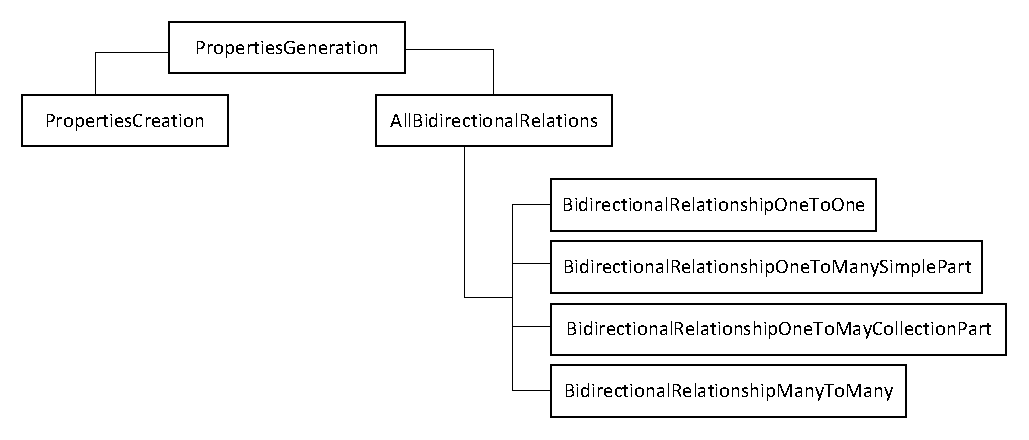
\includegraphics[width=\linewidth]{domainEngineering/images/PropertiesTemplates.eps} \\
  \caption{Orden de ejecuci�n en la plantilla de generaci�n de c�digo \imp{PropertiesGeneration}}
  \label{dom:fig:propTemp}
\end{figure}

Cada plantilla invocada hace uso a su vez de otras subplantillas, que por razones de claridad y espacio no detallamos. Por ejemplo, la plantilla \imp{PropertiesGeneration} encargada de procesar atributos y extremos de asociaci�n, hace uso de diversas plantillas para procesar los extremos pertenecientes a asociaciones doblemente navegables, tal como se indica en la Figura~\ref{dom:fig:propTemp}.

Por �ltimo, comentar que todas las plantillas utilizan diversas funciones auxiliares especificadas en EOL. Por e

\section{Ejemplo de Generaci�n de C�digo C\#: Caso Sencillo}
\label{domain:sec:ejsencillo}
%%==========================================================================%%
%% Author : Abascal Fern�ndez, Patricia                                     %%
%% Author : S�nchez Barreiro, Pablo                                         %%
%% Version: 1.2, 21/04/2013                                                 %%
%%                                                                          %%
%% Memoria del Proyecto Fin de Carrera                                      %%
%% Domain Engineering/Ejemplo de Generaci�n de C�digo C#: Caso Sencillo     %%
%%==========================================================================%%
Para introducir al lector en la implementaci�n de los generadores de c�digo, vamos a analizar en detalle uno de los generadores de c�digo m�s sencillos: \imp{MethodsCreation}, el fichero fuente aparece en el listing \ref{dom:code:method}. Vamos a proceder al an�lisis detallado del mismo:
\begin{itemize}
  \item L�neas 1-3, generadores de c�digo que utiliza y fichero \imp{Operations.eol} que contiene las funciones b�sicas comunes a los generadores de c�digo.
  \item L�nea 4, descripci�n de la funci�n que retornar� el texto generado.
  \item L�nea 6, texto correspondiente al constructor de la clase de la forma $<$nombre del paquete$>$\_init$<$nombre de la clase$>$.
  \item L�neas 8-28, tratamos una a una todas las operaciones descritas en elemento actual (clase o interfaz).
  \item L�neas 9-22, en cada operaci�n recorremos todos y cada uno de los par�metros.
  \item L�neas 11-13, si la operaci�n no tiene definido un tipo, es decir, si el usuario ha obviado especificar si la funci�n devuelve una colecci�n, un entero, un elemento de una clase, etc, por defecto se trata como una operaci�n void (operaci�n que no retorna ning�n valor).
  \item L�nea 15, si la operaci�n tiene un tipo de retorno definido, comprobamos si dicho par�metro es de retorno.
  \item L�nea 16, si el par�metro es de retorno pero no est� definido vuelve a ser tratada como una operaci�n void.
  \item L�nea 18, si el par�metro es de retorno y tiene un tipo definido se trata de una operaci�n que s� retorna un valor.
  \item L�nea 24, si la operaci�n que est� siendo analizada retorna un valor, se a�ade a la lista de operaciones que devuelven un valor.
  \item L�nea 26, si la operaci�n que est� siendo analizada no retorna un valor, se a�ade a la lista de operaciones que no devuelven un valor.
  \item L�nea 29-38, a�adir al string resultado la informaci�n correspondiente a los m�todos de la clase actual que no retornan ning�n valor (m�todos void).
  \item L�nea 31, si el m�todo no tiene un nombre definido, se otorga un nombre por defecto.
  \item L�nea 35, se realizan llamadas a los generadores de c�digo para obtener los par�metros de la funci�n.
  \item L�nea 39-48, de manera an�loga a las operaciones que no retornan ning�n valor, se procede a a�adir al string resultado los m�todos de la clase que s� retornan un valor.
  \item L�nea 49, se retorna el string con todos los m�todos de la clase o interfaz actual.
\end{itemize}

\begin{lstlisting} [basicstyle=\ttfamily\scriptsize,language=CSharp, captionpos=b,
                    caption=Implementaci�n del generador de c�digo \imp{MethodsCreation},
                    label=dom:code:method]
01 [%import "ReturnParameterCreation.egl";
02 import "ParametersCreation.egl";
03 import "../Operations.eol";
04 operation Element classMethods(currentPackage: String, path: String)
                     : String {   		
05  ...
06  opers=private()+void()+currentPackage+"_init"
          +self.firstToUpperCase()+" ( ) {}\n\t\t";
07  ...
08  for (oper in self.getOperations()){
09      for (par in oper.ownedParameter){
10          ...	
11          if (oper.type==null){
12              isReturn=false;
13          }else{
14              if (par.direction.toString().equals("return")){
15                  if (not par.type.name.isDefined()){
16                      isReturn=false;
17                  }else{
18                      isReturn=true;
19                  }//if-par-type
20              }//if-par-direction
21          }//if-oper-type
22      }//for-parameters
23      if (isReturn){
24          operations_return.add(oper);
25      }else{
26          operations_void.add(oper);
27      }		
28  }//for-operations	
29  for (oper in operations_void) {
30      if (oper.name==""){
31          methodname="method_"+iter;
32      }else{
33          methodname=oper.name;
34      }
35      opers=opers+oper.visibility()+oper.abstract()+oper.esStatic()
              +virtual()+void()+currentPackage+"_"+methodname
              +" ("+oper.parameters(currentPackage, path)+") {}\n\t\t";
36      // Increase the iterator
37      iter=iter+1;
38  }
39  for (oper in operations_return) {
40      if (oper.name==""){
41          methodname="method_"+iter;
42      }else{
43          methodname=oper.name;
44      }
45      opers=opers+oper.visibility()+oper.abstract()+oper.esStatic()
             +virtual()+oper.returnParameter(currentPackage, path)
             +" "+currentPackage+"_"+methodname
             +" ("+oper.parameters(currentPackage, path)
             +") {}\n\t\t";
46      // Increase the iterator
47      iter=iter+1;
48  }
49  return opers;
50 }%]
\end{lstlisting}

Un vez explicado un ejemplo sencillo, la siguiente secci�n \ref{domain:sec:ejcomplejo} explica ejemplos m�s complejos que quedan a la curiosidad del lector.



\section{Pruebas}
\label{domain:sec:pruebas}
%%==========================================================================%%
%% Author : Abascal Fern�ndez, Patricia                                     %%
%% Author : S�nchez Barreiro, Pablo                                         %%
%% Version: 1.1, 15/05/2013                                                 %%
%%                                                                          %%
%% Memoria del Proyecto Fin de Carrera                                      %%
%% Application Engineering/Pruebas                                          %%
%%==========================================================================%%

Una vez implementados los generadores de c�digo para la fase de \emph{Ingenier�a de Aplicaciones}, el siguiente paso era dise�ar y ejecutar las pruebas necesarias que permitiesen comprobar el correcto funcionamiento de estos generadores. Para dise�ar las pruebas,  siguiendo el mismo procedimiento que en el caso anterior, utilizando la t�cnica de clases de equivalencia y valores l�mites, para luego completar con casos espec�ficos que permitiesen alcanzar el 100\% de la cobertura.  

A diferencia de la fase de \emph{Ingenier�a del Dominio}, en esta fase no se utiliz� \emph{EUnit} para ejecutar dichas pruebas, ya que dicha herramienta no se ajustaba a nuestras necesidades. Por tanto, se crearon los casos de prueba y se ejecutaron a mano, analizando de forma tambi�n manual si la salida producida coincid�a con la esperada. La Tabla~\ref{app:table:pruebas} muestra algunos de los casos de prueba ejecutados.

\begin{table}
\begin{small}
\begin{tabularx}{\linewidth}{|X|l|}
 \hline
{Casos v�lidos}&{Casos no v�lidos} \\ \hline
Configuraci�n con un solo camino hoja-raiz & Paquetes recursivos. \\
Configuraci�n con varios caminos y todos los m�todos independientes &\\
Configuraci�n con varios caminos y alg�n m�todo dependiente &\\
Configuraci�n con varios caminos, donde alg�n m�todo tiene versiones dependientes e independientes &\\
\hline
\end{tabularx}
\end{small}
\caption{Casos de prueba para la fase de Ingenier�a de la Aplicaci�n}
\label{app:table:pruebas}
\end{table}%

Una vez creados y probados los generadores de c�digo, el siguiente paso era empaquetarlos para posibilitar su distribuci�n y uso. La siguiente secci�n describe como se realiza dicha fase de despliegue.
Tras ejecutar estos casos de prueba y comprobar que los generadores de c�digo funcionaban correctamente, d�bamos por concluida la labore de desarrollo de los generadores de c�digo, restando solo su empaquetado y despliegue.



\section{Sumario}

Durante este cap�tulo se ha descrito el proceso de desarrollo de los generadores de c�digo para la fase de \emph{Ingenier�a del Dominio} de la metodolog�a Te.Net. Para ello, primero se ha analizado c�mo se transforman los elementos de un modelo UML 2.0 orientado a caracter�sticas en c�digo C\#. A continuaci�n, se ha descrito de forma superficial la implementaci�n de los generadores de c�digo, mostrando el funcionamiento de una sencilla plantilla. Por �ltimo, se han descrito las pruebas realizadas.
